% This is samplepaper.tex, a sample chapter demonstrating the
% LLNCS macro package for Springer Computer Science proceedings;
% Version 2.21 of 2022/01/12
%
\documentclass[runningheads]{llncs}
%
\usepackage[T1]{fontenc}
\usepackage{amsmath} 
% T1 fonts will be used to generate the final print and online PDFs,
% so please use T1 fonts in your manuscript whenever possible.
% Other font encondings may result in incorrect characters.
%
\usepackage{graphicx}
\bibliographystyle{splncs04}

% Used for displaying a sample figure. If possible, figure files should
% be included in EPS format.
%
% If you use the hyperref package, please uncomment the following two lines
% to display URLs in blue roman font according to Springer's eBook style:
%\usepackage{color}
%\renewcommand\UrlFont{\color{blue}\rmfamily}
%\urlstyle{rm}
%
\begin{document}
%
\title{Benchmarking of zk-STARK and zk-SNARK in Privacy-Preserving Federated Learning Scenario}
%
%\titlerunning{Abbreviated paper title}
% If the paper title is too long for the running head, you can set
% an abbreviated paper title here
%
\author{Lars Blütecher Holter\inst{1}\orcidID{0009-0004-0932-4447}}
%
\authorrunning{Lars Blütecher Holter}
% First names are abbreviated in the running head.
% If there are more than two authors, 'et al.' is used.
%
\institute{Norwegian University of Science and Technology - NTNU, Norway 
\email{larsern99@hotmail.com}}
%
\maketitle              % typeset the header of the contribution
%
\begin{abstract}
Sharing sensitive information for the purpose of building machine learning models is often prohibited due to technical, legal, or privacy aspects. Federated learning is a technology where distributed participants collaborate to build machine learning models while at the same time protecting sensitive private information. The challenge is to enable distributed computing without sharing data. One of the solutions is in non-interactive zero-knowledge proof algorithms. 
Zero-knowledge proofs enable verification of computational correctness without revealing private data, and thus zero-knowledge technology addresses critical privacy challenges in federated learning. 
Although zk-SNARKs have been applied to federated learning systems, no empirical comparison between zk-SNARKs and zk-STARKs has been conducted, and thus we provide an evaluation framework for benchmarking zero-knowledge algorithms in a federated learning scenario. Our experiments demonstrate that zk-STARKs outperform zk-SNARKs for privacy-preserving federated learning applications, achieving significant performance advantages.
The implementation of zk-STARK exhibits sublinear $O(n log n)$ scaling characteristics, requiring only $14.37$ seconds for the batch size of $40$, while zk-SNARKs demonstrate $O(n^{2})$ behavior, with $1011.68$ seconds for the same workload. Memory efficiency analysis reveals that zk-STARKs consume $2.9 \times$ to $6.4 \times$ less memory. 
Although zk-STARK proofs are larger ($1359 \times$ to $1671 \times$ the size of zk-SNARK proofs), this trade-off becomes increasingly acceptable for computationally intensive applications where the performance gains outweigh storage costs.

\keywords{zero-knowledge \and zk-STARK \and blockchain \and federated learning \and zk-SNARK \and benchmark}
\end{abstract}


% ==============================
\section{Introduction}

Federated learning, introduced by Google in 2016, enables collaborative model training without sharing raw data by distributing computations across decentralized devices~\cite{googlefederated2016}. 
However, FL systems remain vulnerable to malicious participants who may submit invalid model updates designed to poison the global model, or honest but curious participants may extract private information.
Existing FL frameworks have integrated zk-SNARKs to enforce verifiable training and aggregation~\cite{mainflzkp,msthesis}, but these implementations face challenges: (i) zk-SNARKs require a trusted setup that creates potential security vulnerabilities, (ii) due to the reliance on elliptic curves they are not quantum safe, and (iii) exhibit poor scaling as model complexity increases, making proof generation prohibitively expensive for complex AI workloads.

In contrast, zk-STARKs employ a transparent setup that eliminates trust assumptions and offer quasi-linear scaling in proof generation time. In addition, the underlying technology relies on collision-resistant hash functions and the FRI protocol, providing post-quantum security guarantees.
Theoretical analysis suggests that zk-STARKs are potentially better suited for AI-centric workloads~\cite{oude2024systematic}. 
However, despite these theoretical predictions, no prior work has implemented a complete zk-STARK-based FL system and directly compared its performance to zk-SNARKs. 
Our work addresses this research gap by providing a comprehensive empirical evaluation of zk-STARK versus zk-SNARK in federated learning.

Our contributions include: (1) proof-of-concept implementation of federated learning using zk-STARKs that provides empirical comparison between two zero-knowledge algorithms, zk-STARKS and zk-SNARKs; (2) custom AIR constraints encoding neural network operations for privacy-preserving federated learning; (3) comprehensive performance analysis demonstrating $70 \times$ speedup and superior memory efficiency; (4) validation of theoretical predictions about zk-STARK superiority for computationally intensive AI applications.



% ========================================
\section{Background and Related Work}

%\subsection{Zero-Knowledge Proof Systems}
zk-SNARKs provide compact proofs with fast verification.
However, they require a trusted setup where cryptographic parameters are generated, e.g.~through multi-party computation~\cite{firstzksnark}.
If participants retain secret randomness from the trusted setup, so-called toxic waste, they could forge proofs, compromising system security. {\tt Groth16} produces constant-size proofs regardless of computation complexity~\cite{groth16}, but reliance on elliptic curves introduces potential vulnerability to quantum attacks.

zk-STARKs eliminate the need for trusted setup, and use collision-resistant hash functions and the FRI protocol. The transparent setup ensures that participants can independently verify the system parameters without trusting external parties. zk-STARKs provide post-quantum security, since they depend on hash functions rather than number-theoretic assumptions vulnerable to quantum attacks.

% \subsection{Federated Learning with Zero-Knowledge Proofs}

Haimerl's thesis presented a blockchain-based FL architecture using zk-SNARKs for on-chain verification~\cite{msthesis}. IoT edge devices compute local updates and generate zk-SNARK proofs submitted to an Ethereum smart contract.
The implementation demonstrated zero-knowledge integration, but faced scalability challenges due to high gas costs and quadratic scaling in circuit compilation.

Ebrahimi et al.~developed VeriBlock-FL, that can perform proof generation off-chain while maintaining on-chain verification~\cite{mainflzkp}. This design reduces gas costs but still faces fundamental scalability limitations due to the underlying zk-SNARK technology.

A systematic literature review by Oude Roelink et al.~found 31 zk-SNARK deployments and none zk-STARK implementations in practical systems~\cite{oude2024systematic}.
Although El-Hajj et al.~benchmarked zk-SNARKs and zk-STARKs using MiMC hash computations, their evaluation used only simplified circuits rather than realistic AI workloads~\cite{evaluatingzkp}.


% ========================================
\section{System Design and Implementation}

\subsection{Architecture Overview}
Our system implements an off-chain federated learning framework where clients generate zk-STARK proofs for local training, and the aggregator produces verifiable proof for averaging and aggregating local models. The use of zk-STARKs for both, training and aggregation, eliminates blockchain overheads.
The setup also enables us to compare zk-SNARKs and zk-STARKs in a realistic federated learning workload. 

The system workflow follows these key steps:
\begin{enumerate}
\item \textbf{Train local model \& generate zero-knowledge proof}: Each client performs local training using the neural network implementation and generates a zk-STARK proof using the {\tt TrainingUpdateAir} constraints.
\item \textbf{Send local model \& and the proof}: Clients transmit their model updates along with the corresponding ZKPs directly to the aggregator. There is no need for any blockchain infrastructure.
\item \textbf{Verify ZKPs off-chain}: The aggregator validates all received proofs, ensuring the computational integrity of local models. This allows the aggregator to verify the data before aggregating, and without accessing any private data.
\item \textbf{Update global model \& generate ZKP}: Using the federated averaging algorithm ({\tt FedAvg}), the aggregator computes a new global model and generates its own proof for the aggregation process.
\item \textbf{Distribute updated global model}: The aggregator sends the updated global model along with the proof back to all participating clients for the next training round.
Cients can also verify that the aggregation was done correctly. 
\end{enumerate}

This design ensures that every computational step is cryptographically verifiable while maintaining complete privacy of local training data, as illustrated in Figure~\ref{fig:system_overview}.

\begin{figure}[ht]
\centering
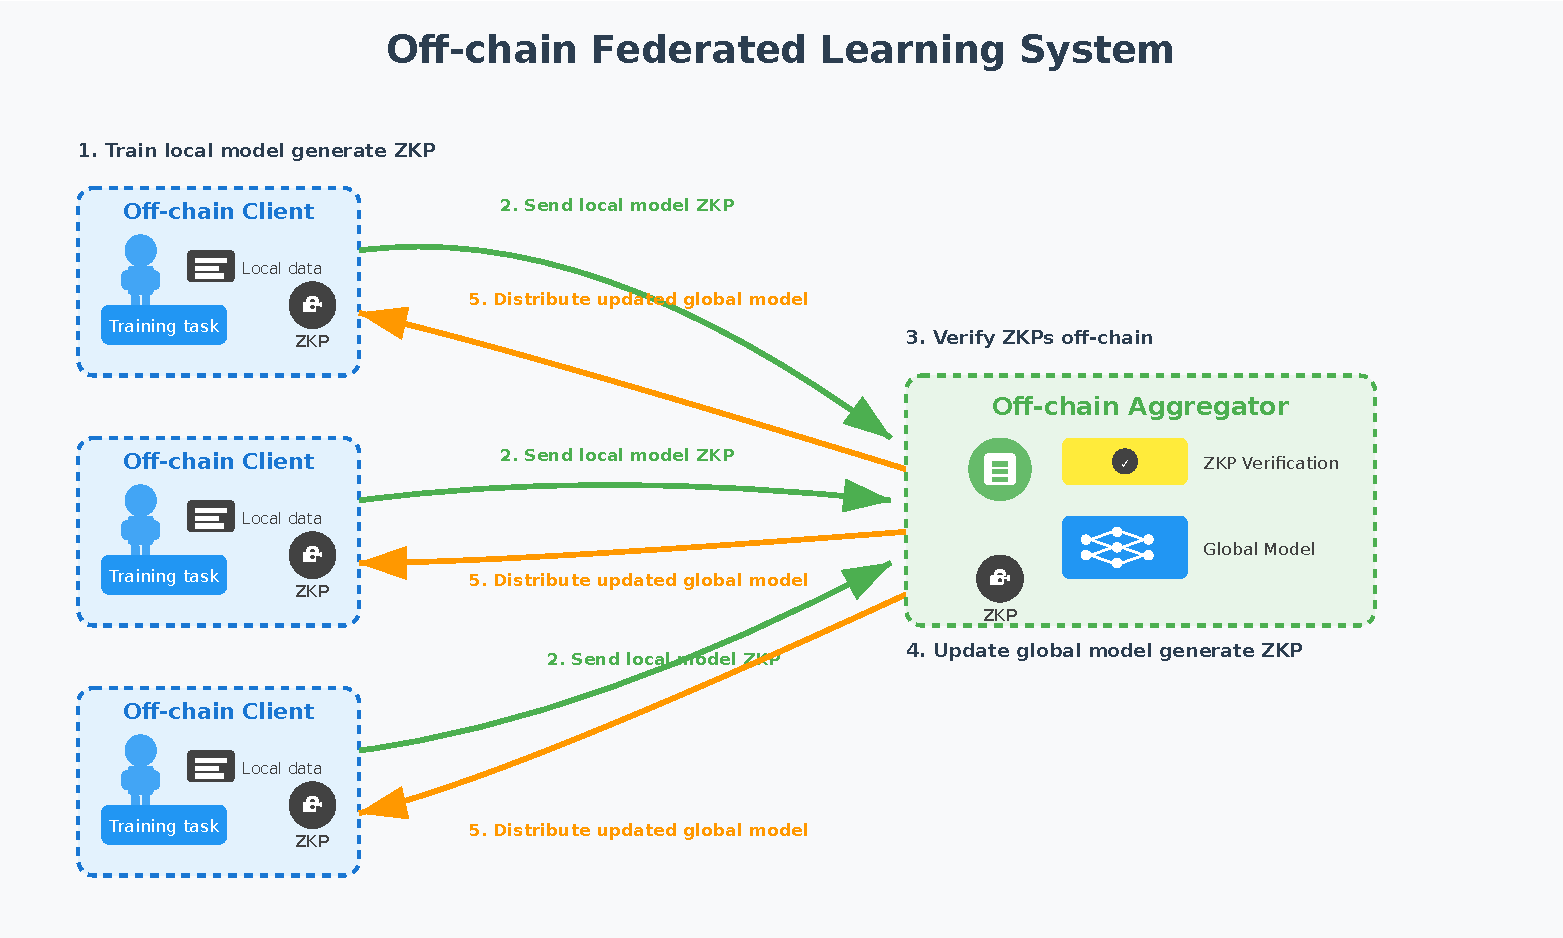
\includegraphics[width=\textwidth]{offchain_fl_system.pdf}
\caption{Overview of the off-chain federated learning system}
\label{fig:system_overview}
\end{figure}

% ========================================
\subsection{zk-STARK Implementation}

Our zk-STARK system is implemented in {\tt Rust} and uses the {\tt Winterfell} library.
Our implementation relies on two custom Arithmetic Intermediate Representation (AIR) modules encoding federated learning computational constraints.

\textbf{TrainingUpdateAir} encodes local stochastic gradient descent (SGD) operations, including forward propagation, backward propgation, and gradient descent.
The core constraint ensures correct parameter updates:
\[
\text{weight}^{(t)} - \text{gradient} \cdot \eta - \text{weight}^{(t+1)} = 0
\]

\textbf{GlobalUpdateAir} encodes federated averaging, enforcing constraints like:
\[
k \times \text{new\_global} - k \times \text{global} - \text{update} = 0
\]
where $k$ is the scaling factor for aggregation.


% ==========================================
\subsection{Finite Field Arithmetic}

A critical challenge for using zk-STARKs is the representation of real-valued parameters within finite fields.
We have developed a fixed-point encoding using a scaling factor $10^6$ and a signed-pair representation $(|v|, \text{sign})$. A cleanse function maps signed pairs to field elements:
\[
\text{cleanse}(m, s) = \begin{cases}
m & \text{if } s = 0 \\
\text{MAX} - m + 1 & \text{if } s = 1
\end{cases}
\]

We implemented generic arithmetic operations handling sign propagation correctly while maintaining computational correctness in finite field operations.



% ================================================
\subsection{Zero-Knowledge Properties}

We achieve zero-knowledge through one-time pad masking that conceals model parameters while preserving computational relationships.
Masking is applied through field addition: $\text{masked\_param} = \text{original\_param} + \text{random\_mask}$. Since masks are uniformly distributed, this provides information-theoretic privacy guarantees.



% =================================================
\section{Experimental Setup}

For the experiments we have used the {\em Daily and Sports Activities} dataset containing IoT sensor data~\cite{daily_and_sports_activities_256}.
Following VeriBlock-FL methodology, we reduced features from $45$ to $9$ dimensions and consolidated $19$ activities to $6$ categories. We used a single-layer neural network with $9$ inputs and $6$ outputs.

Our benchmarking framework conducted systematic evaluation across batch sizes between $1$ to $40$, executing each configuration 11 times to obtain statistical reliability.
We measured execution time (total and phase-wise), memory consumption (peak and average), and recorded the proof sizes.
For zk-SNARK comparison, we used the VeriBlock-FL codebase with identical parameters.

The framework implements multiple timing sources, memory monitoring through application and system-level tools, automated outlier detection using z-score methodology, and statistical analysis including confidence intervals.

All experiments used MacBook Pro (2023) with Apple M2 Pro processor, 16 GB memory, running macOS Sequoia 15.4.1.


% ===========================================
\section{Results and Analysis}

\subsection{Overall Performance}

Our evaluation reveals significant performance advantages for zk-STARKs across all batch sizes. At batch size 1, zk-STARKs complete in $4.71\pm3.6\%$ (coefficient of variance, CV, reported as percentage) seconds versus $9.91\pm0.36\%$ seconds for zk-SNARKs ($2.1 \times$ speedup).

\begin{figure}[htbp]
    \centering
    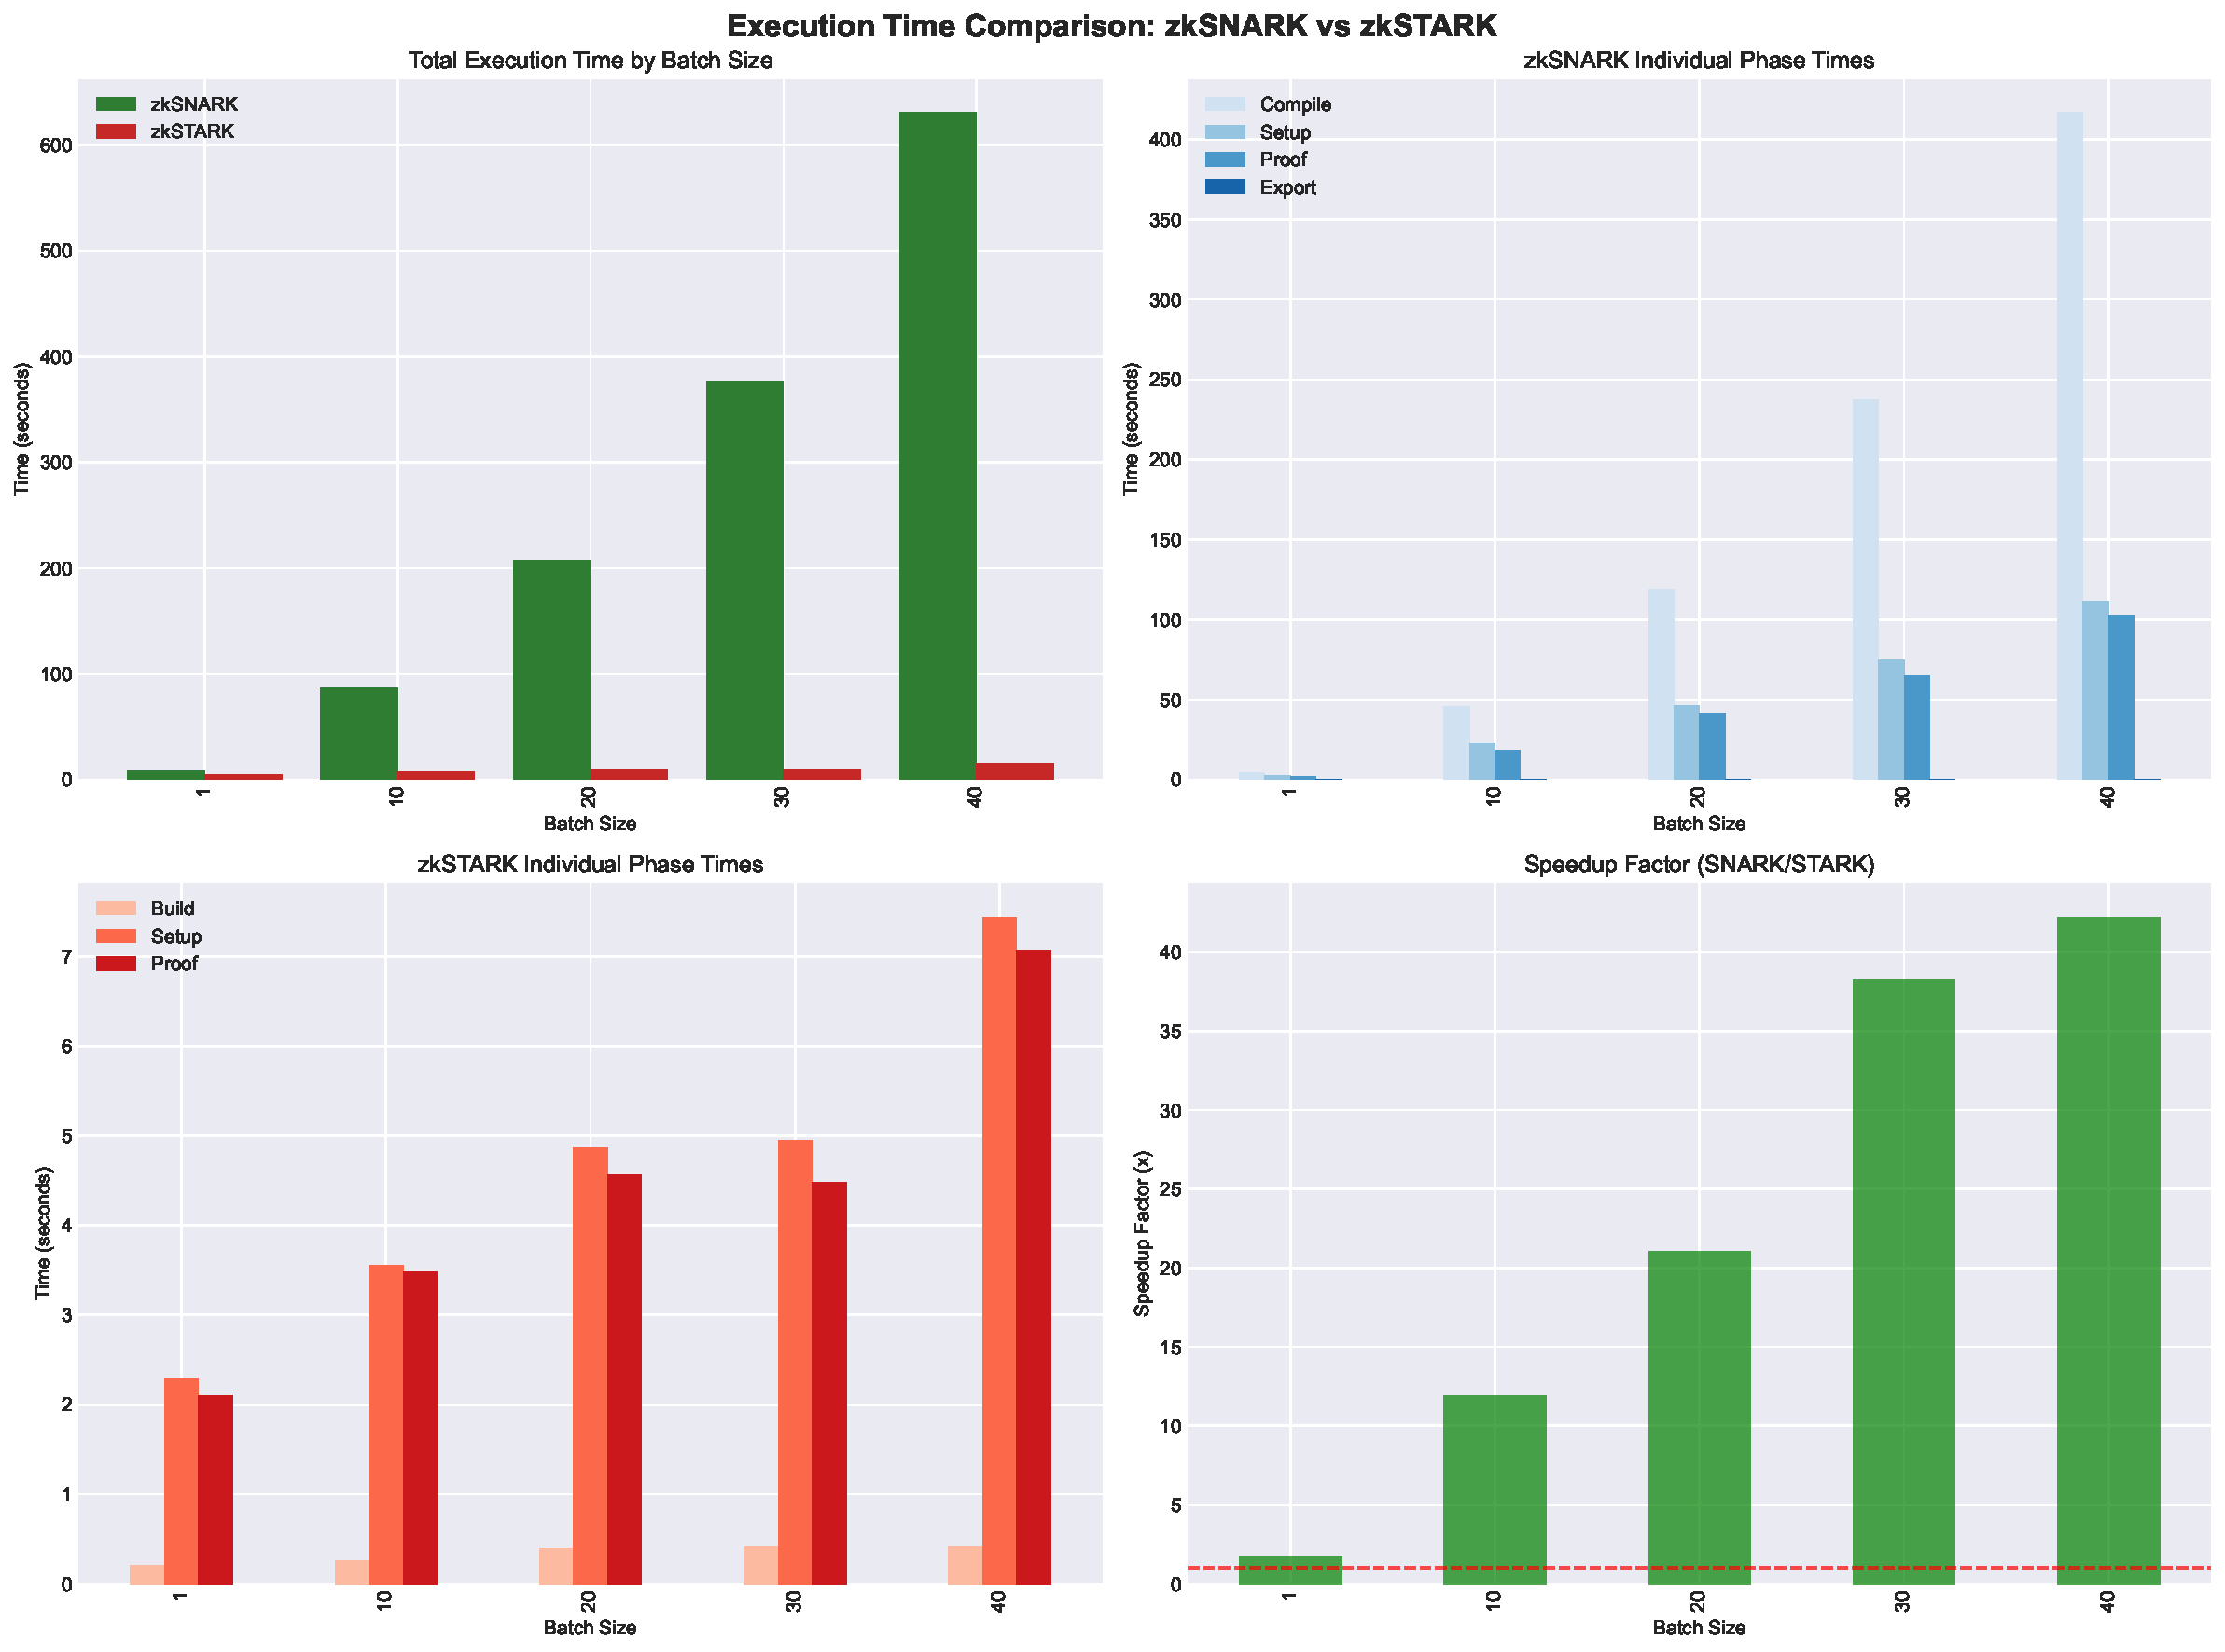
\includegraphics[width=0.9\textwidth]{time_comparison.pdf}
    \caption{Execution time comparison between zk-SNARK and zk-STARK systems across different batch sizes, showing total time and phase-wise breakdown.}
    \label{fig:time_comparison}
\end{figure}

This gap widens substantially at batch size 40, where zk-STARKs require only $14.37\pm4.3\%$ seconds while zk-SNARKs need $1011.68\pm0.41\%$ seconds, yielding a \textbf{$70.4 \times$ speedup}.

zk-STARK execution demonstrates sub-linear scaling, growing only $3.0 \times$ across the tested range, consistent with $O(n log n)$ complexity. zk-SNARKs exhibit polynomial scaling, increasing $102 \times$ and approaching $O(n^{2})$ scaling behavior.

\begin{figure}[htbp]
    \centering
    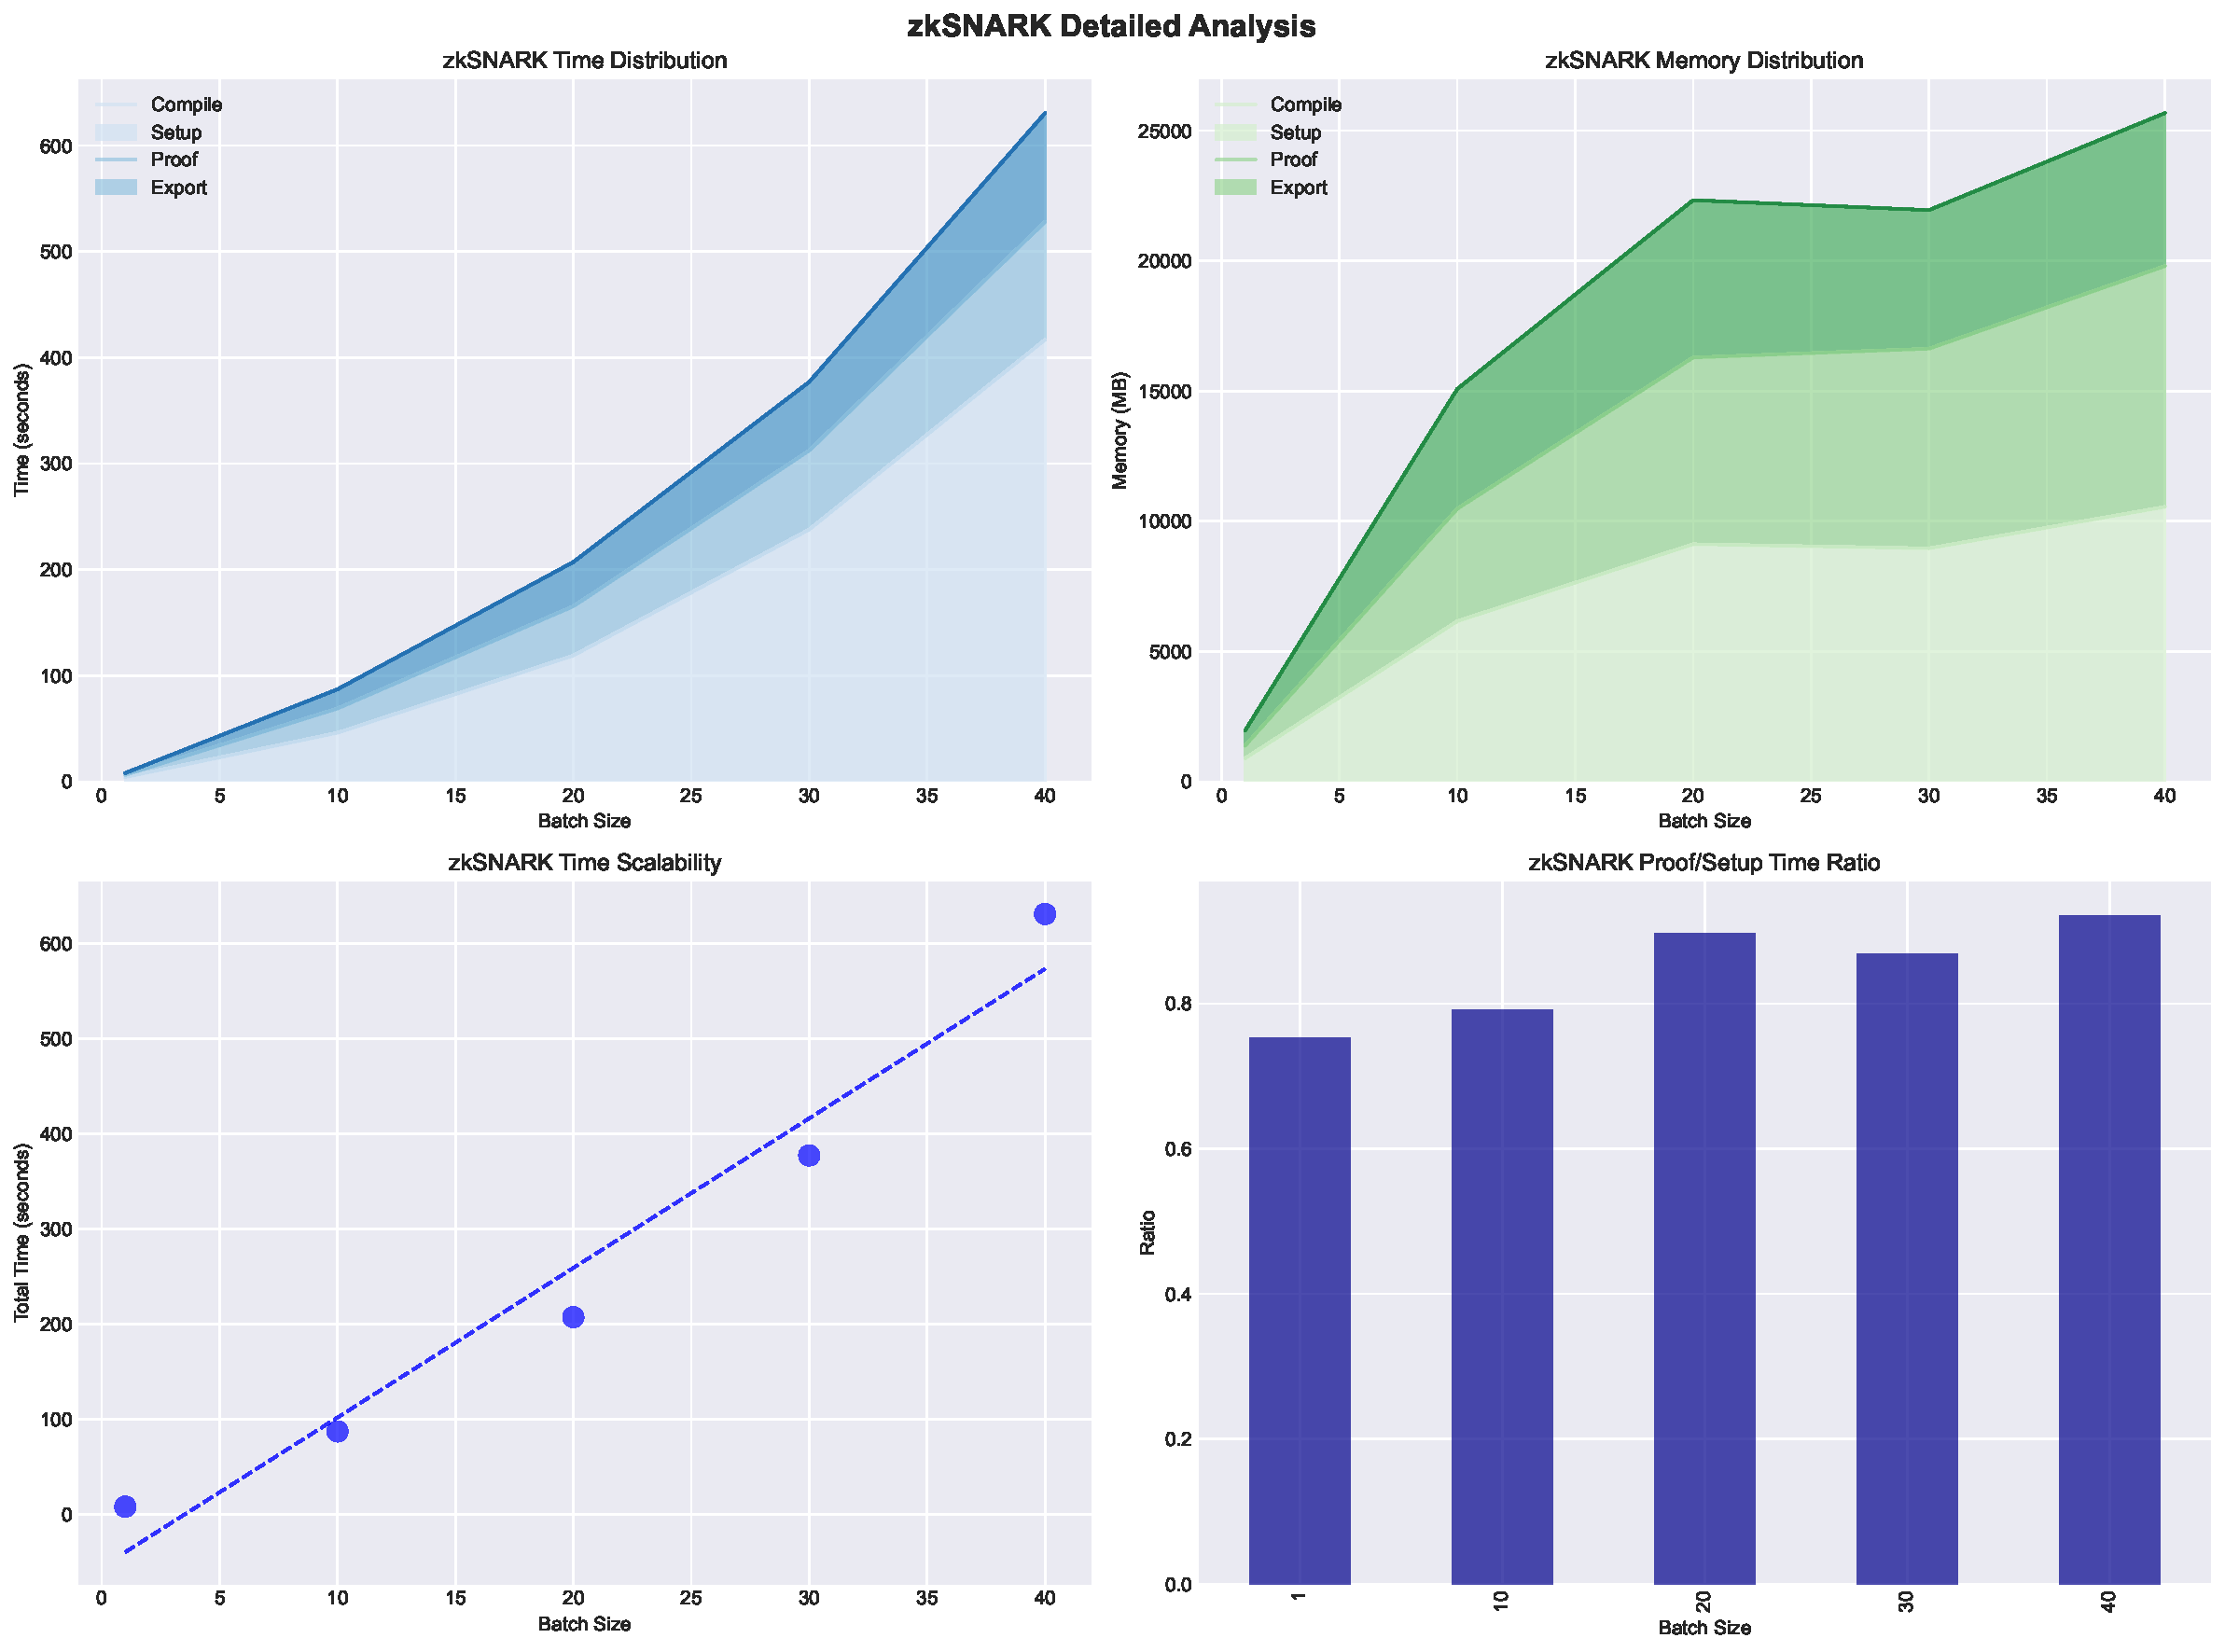
\includegraphics[width=0.9\textwidth]{snark_detailed.pdf}
    \caption{Detailed analysis of zk-SNARK performance showing time and memory distribution across different phases (compile, setup, proof, export) and scalability characteristics.}
    \label{fig:snark_detailed}
\end{figure}

% ===========================================
\subsection{Phase-Level Analysis}

For zk-SNARKs, compilation emerges as the primary bottleneck, escalating from $4.83$ seconds (batch 1) to $717.47$ seconds (batch 40).
This represents $149\times$ increase representing 70.9\% of total execution at scale. Setup grows from $2.49$ to $146.65$ seconds ($59\times$ increase), while proof generation increases from $1.82$ to $122.89$ seconds ($68\times$ increase).

zk-STARKs maintain balanced performance across phases. Build phase increases minimally from $0.21$ to $0.45$ seconds ($2.1\times$ increase). Setup and proof phases show controlled growth: 3.2× ($2.25$ to $7.17$ seconds) and $3.0\times$ ($2.25$ to $6.75$ seconds) respectively, with no single phase dominating.



\subsection{Memory Efficiency}

\begin{figure}[htbp]
    \centering
    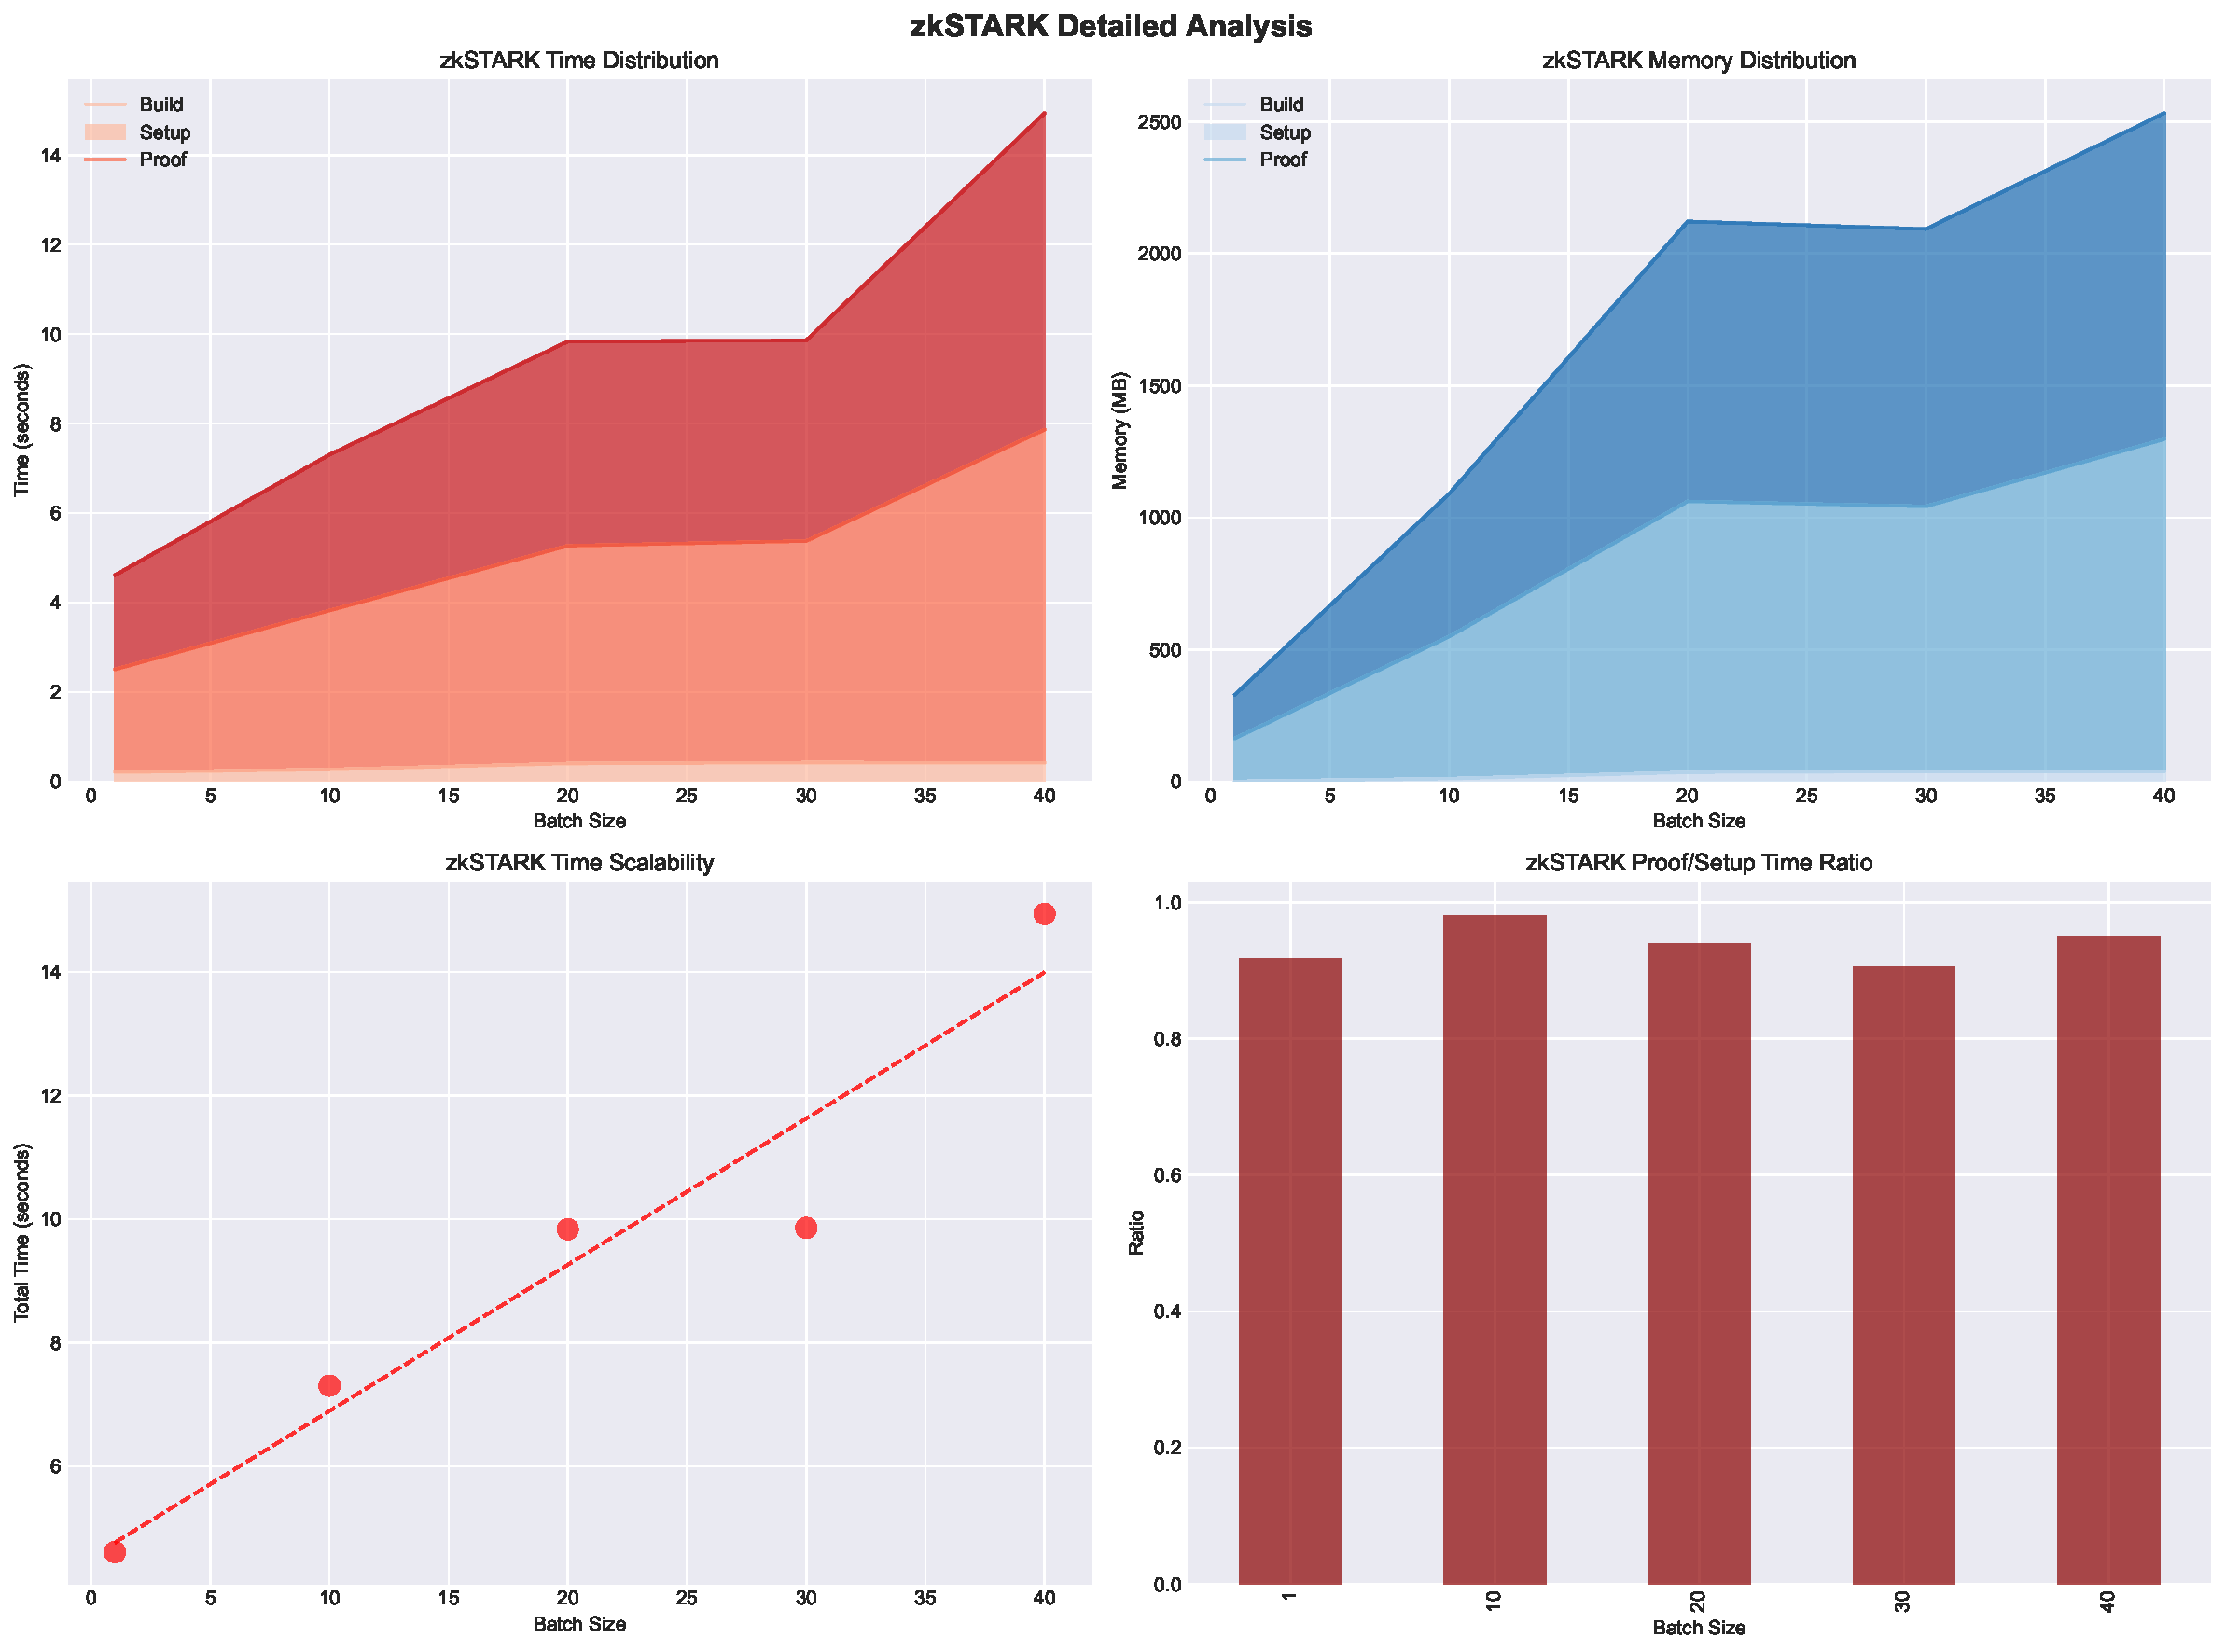
\includegraphics[width=0.8\textwidth]{stark_detailed.pdf}
    \caption{Detailed analysis of zk-STARK performance showing time and memory distribution across different phases (build, setup, proof) and scalability characteristics.}
    \label{fig:stark_detailed}
\end{figure}

zk-STARKs consistently require $2.9\times$ to $6.4\times$ less memory than zk-SNARKs. At batch size 40, zk-STARKs peak at $1.42$~GB compared to $6.25$~GB for zk-SNARKs. Memory scaling favors zk-STARKs with controlled logarithmic growth (setup increases $8.8\times$), while zk-SNARKs exhibit near-polynomial scaling (setup increases $10.9\times$) creating severe resource requirements.

\subsection{Proof Size Trade-offs}

The primary zk-STARK disadvantage is the proof size. zk-STARK proofs range from $1.48$ MB to $1.91$ MB, representing $1359\times$ to $1671\times$ larger than zk-SNARKs (always under $1$~KB). However, proof size growth is sub-linear: despite 40× computational increase, zk-STARK proof size increases only $29.1\%$.

In federated learning scenarios where verification frequency is low relative to proof generation, computational efficiency gains significantly outweigh storage costs. Clients generate proofs continuously but verification occurs only during periodic aggregation.


\subsection{Validation of Intrinsic Performance}

To ensure performance differences stem from algorithmic characteristics rather than implementation artifacts, we analyzed zk-SNARKs excluding compilation.
Even optimized, zk-STARKs maintain substantial 20.5× advantage ($14.4$ vs $294.2$ seconds at batch size $40$), confirming intrinsic superior scaling.

Statistical reliability analysis shows consistent measurements across both systems. zk-STARKs demonstrate moderate temporal variance (CV $2.3\%$ to $5.1\%$) and stable memory variance, while maintaining highly consistent proof sizes (CV under $0.5\%$).




\section{Discussion and Implications}

{\bf Performance Implications}. The empirical evidence validates theoretical predictions about zk-STARK superiority for AI applications. The performance advantages demonstrate transformative differences that fundamentally alter privacy-preserving computation viability at scale.
Memory efficiency characteristics enable deployment on standard infrastructure without specialized hardware, making privacy-preserving AI accessible to resource-constrained organizations.

The transparent setup eliminates operational complexity and security vulnerabilities from trusted setup ceremonies. Combined with post-quantum security, these characteristics position zk-STARKs as superior for applications requiring long-term security assurance.


{\bf Scalability and Cost-Benefit Analysis}.
Sub-linear scaling characteristics suggest zk-STARKs become increasingly advantageous as AI models grow in complexity—precisely modern AI development trajectory. Organizations operating large-scale privacy-preserving AI systems would realize substantial cost savings from 70.4× computational reduction, even accounting for additional storage costs.

The demonstrated efficiency improvements translate to significant energy savings supporting environmentally sustainable deployment of privacy-preserving AI technologies. The implementation using general-purpose programming languages demonstrates practical viability across diverse systems and platforms.


{\bf Practical Deployment Considerations}.
For applications where verification frequency is low relative to proof generation—typical in federated learning—computational efficiency gains significantly outweigh storage costs. The sub-linear proof size growth suggests this trade-off becomes increasingly favorable as system scale increases.

Balanced phase performance indicates robust scalability without algorithmic bottlenecks that would limit applicability to complex workloads. This positions zk-STARKs as foundational technology for next-generation privacy-preserving AI systems that can scale to meet demands of increasingly complex machine learning applications.


% ==========================================
\section{Limitations}

%Our evaluation used simplified neural networks that may not reflect production-scale complexity. The off-chain focus limits insights into blockchain deployment where gas costs matter. Apple Silicon architecture may not represent x86 performance characteristics, and single library usage means library-specific optimizations may influence results.

%Future work should extend to blockchain integration for cost-benefit analysis, cross-platform evaluation on x86 architectures, and investigation of the performance anomaly at batch size 30. Evaluation with complex neural architectures would provide insights into realistic AI workload scaling.


This study acknowledges several limitations affecting the interpretability and generalizability of its findings.

{\bf Internal Validity}.

{\em Implementation asymmetries:} The zk-SNARK baseline utilized ZoKrates (a high-level toolkit), while the zk-STARK implementation employed Winterfell in Rust. Toolchain differences may introduce performance variations unrelated to protocol efficiency.

{\em Simplified arithmetic:} Signed arithmetic in finite fields was implemented via fixed-point encoding rather than bit decomposition, potentially inflating constraint complexity.

{\em Neural network simplicity:} The single-layer architecture (9 inputs $\times$ 6 outputs) does not reflect computational demands of deep learning models.

{\bf External Validity}.

{\em Dataset constraints:} Experiments used the {\em Daily and Sports Activities} dataset (9 features, 6 classes), limiting extrapolation to high-dimensional data (e.g., images, text).

{\em Hardware specificity:} Benchmarks executed exclusively on Apple M2 Pro (ARM architecture); results may differ on x86 CPUs or GPUs.

{\em Scale limitations:} Batch sizes capped at 40 samples; behavior at web-scale FL (1,000+ clients) remains unverified.

{\bf Reliability}.

{\em Statistical robustness:} Eleven runs per configuration ensured stable central estimates ($CV < 5.1\%$ for temporal metrics), but rare anomalies (e.g., the $5.7\%$ runtime dip for zk-STARKs at batch 30) warrant further investigation.

{\em Environmental consistency:} Memory monitoring relied on macOS APIs; cross-platform verification is needed to exclude OS-specific artifacts.

These limitations constrain direct extrapolation to industrial-scale FL but establish a foundational framework for future benchmarking.



% =============================================
\section{Conclusion}

Our work provides a comprehensive empirical validation of zk-STARK performance as compared to zk-SNARKs in privacy-preserving federated learning.
Our systematic evaluation demonstrates transformative performance advantages, 70.4× speedup and 2.9× to 6.4× memory efficiency—while providing transparent setup and post-quantum security.

The sublinear scaling characteristics make zk-STARKs optimal for AI applications where computational demands continue to grow. While proof sizes remain larger, demonstrated efficiency gains outweigh storage costs for large-scale applications, particularly as the relative penalty grows sub-linearly.

These findings challenge prevailing assumptions about zero-knowledge proof selection and suggest a paradigm shift for computationally intensive applications. The work establishes zk-STARKs as the preferred technology for privacy-preserving machine learning requiring scalability and performance, with implications extending to any domain requiring privacy-preserving verification of complex computations.

%\section{Acknowledgements}
%I sincerely thank Professor Mariusz Nowostawski for invaluable supervision and Meriem Guerar for introducing and guiding me through federated learning topics and ZKP applications during this research.




%
% ---- Bibliography ----
%
% BibTeX users should specify bibliography style 'splncs04'.
% References will then be sorted and formatted in the correct style.
%

\bibliography{references}

\end{document}
